% vim:syntax=tex

In this section we provide an overview of the document extraction and retreival process
used for feature location.
We also provide an overview of two topic models,
latent semantic indexing (LSI) and latent Dirichlet allocation (LDA),
and review closely related work.

\subsection{Feature Location Techniques} % oh wtf


\begin{figure*}
\vspace{2mm}
\centerline{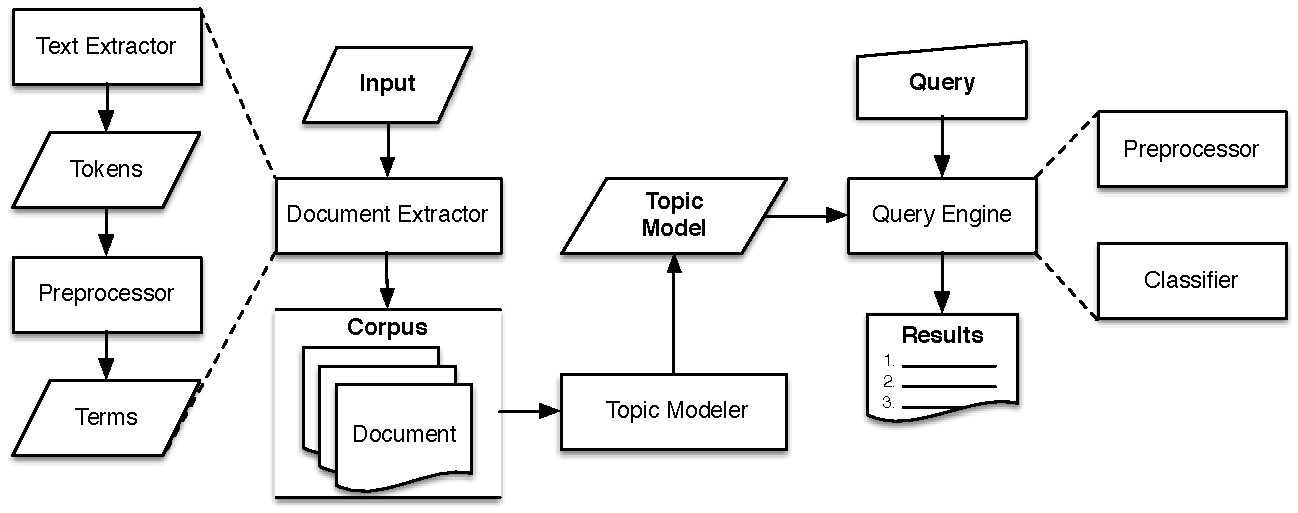
\includegraphics[width=.8625\textwidth]{figures/Process}}
\caption{The general document extraction and retrieval process.}
\label{fig:process}
\vspace{-2mm}
\end{figure*}


\subsubsection{Snapshots}

A \textit{word} is the basic unit of discrete data in a software lexicon and is a sequence of letters.
A \textit{token} is a sequence of non-whitespace characters containing one or more words.
An \textit{entity} is a named source element such as a method,
and an \textit{identifier} is a token representing the name of an entity.
\textit{Comments} and \textit{literals} are sequences of tokens delimited by language-specific markers (e.g., /* */ and quotes).
The \textit{document} which corresponds to a class is a sequence of words $d = (w_1, \ldots, w_m)$,
and a \textit{corpus} is a set of documents (i.e., classes) $D = (d_1, \ldots, d_n)$.

The left side of Figure~\ref{fig:process} illustrates the document extraction process.
A document extractor takes source code as input and produces a corpus as output.
Each document in the corpus contains the words associated with a class.
The text extractor is the first part of the document extractor.
It parses the source code and produces a token stream for each class.
The preprocessor is the second part of the document extractor.
It applies a series of transformations to each token and
produces one or more words from the token.
The transformations~\cite{Marcus-etal:2004,Marcus-Menzies:2010}: % that we use are:
\begin{itemize}
    \item {\it Splitting}: separate tokens into constituent words
        based on common coding style conventions (e.g., the use of camel case or underscores)
        and on the presence of non-letters (e.g., punctuation or digits)
    \item {\it Normalizing}: replace each upper case letter with the corresponding
        lower case letter
    \item {\it Filtering}: remove common words such as articles (e.g., `an' or `the'),
        programming language keywords, standard library entity names, or short words
\end{itemize}

The right side of Figure~\ref{fig:process} illustrates the retrieval process.
Once a topic model has been built, it can be used as part of a query engine.
The query engine's job is to take a query and infer how it relates to topics in the model.
Additionally, it can classify, or rank, the results of this inference to another inference.
That is, the classifier step finds other documents that have similar topics in the model.


\subsubsection{Changesets}

A \textit{diff} is a set of text which represents the differences between two texts.
A \textit{patch} is a set of instructions (i.e., diffs) that can be used to transform one text into another.
\textit{Context lines} denote text useful for transforming the text, but do not represent the differences.
\textit{Added lines} are lines which were added in order to transform the first text into the second.
Similarly, \textit{removed lines} are lines which are removed for this same purpose.
Figure~\ref{fig:diff} shows an example of what a changeset might look like.
A \textit{changeset}, ideally, represents a single feature modification, addition, or deletion, which may crosscut many source code entities.
The terms changeset and patch are often used interchangeably.

For changesets, the document extraction process remains mostly the same.
However, instead of extracting documents by parsing source code for identifiers, comments, and literals,
the changeset itself is parsed.
In a changeset, it may be desirable to parse further for source code entities.
The same preprocessor transformations may also occur in changesets.

To leverage the online functionality of the topic models,
we can intermix the document extraction and retrieval steps.
First, we initialize a model in online mode.
Then, as changes are made, the model is updated with the new changeset.
Next, we can use a dynamic programming to update $\theta_{snapshot}$
with new inferences of source code documents affected by this changeset.
Now the model is current with the latest source code.
We can then query the model as needed and rank the results of that query
against $\theta_{snapshot}$.
Note that we never care about infering a $\theta_{changeset}$ for documents on which the model is built.


%diff --git a/lao b/tzu
%index 635ef2c..5af88a8 100644
%--- a/lao
%+++ b/tzu
\begin{figure}[ht]
\centering
\footnotesize
\begin{lstlisting}[language=diff, basicstyle=\ttfamily]
--- lao
+++ tzu
@@ -1,7 +1,6 @@
-The Way that can be told of is not the eternal Way;
-The name that can be named is not the eternal name.
 The Nameless is the origin of Heaven and Earth;
-The Named is the mother of all things.
+The named is the mother of all things.
+
 Therefore let there always be non-being,
   so we may see their subtlety,
 And let there always be being,
@@ -9,3 +8,6 @@ And let there always be being,
 The two are the same,
 But after they are produced,
   they have different names.
+They both may be called deep and profound.
+Deeper and more profound,
+The door of all subtleties!
\end{lstlisting}
\caption{Example of a \texttt{git diff}.
Black or blue lines denote metadata about the change useful for patching.
In particular, black lines represent context lines (beginning with a single space).
Red lines (beginning with a single~\texttt{-}) denote line removals,
and green lines (beginning with a single~\texttt{+}) denote line additions.}
\label{fig:diff}
\vspace{-10pt}
\end{figure}


\subsection{Latent Semantic Indexing}

Latent semantic indexing~\cite{Deerwester:1990} is an indexing and
retrieval methodolgy. LSI uses a statistical technique, singular value
decomposition to identify patterns within the unstructured data. That is,
LSI identifies relationships between terms and documents, and places
documents that are related close to one another creating a semantic space.


\subsection{Latent Dirichlet Allocation}

Latent Dirichlet allocation~\cite{Blei-etal:2003} is a generative topic model.
LDA models each document in a corpus of discrete data as a finite mixture over a set of topics
and models each topic as an infinite mixture over a set of topic probabilities.
That is, LDA models each document as a probability distribution
indicating the likelihood that it expresses each topic and
models each topic that it infers as a probability distribution
indicating the likelihood of a word from the corpus being assigned to the topic.

Inputs to LDA include a corpus and $K$, the number of topics.
LDA represents each document in the corpus as a bag-of-word (multiset)
and thus disregards word order and structure.
Outputs of LDA include $\phi$, the term-topic probability distribution,
and $\theta$, the topic-document probability distribution.


\subsection{Feature Location}

